\documentclass[10pt]{beamer}

\usetheme{metropolis}

\usepackage{fontspec}
\setsansfont[BoldFont={Fira Sans SemiBold}]{Fira Sans Book}
\setsansfont{Fira Sans}
\setmonofont{Fira Mono}

\usepackage{appendixnumberbeamer}

\usepackage{booktabs}

\title{EL 1207 - Rangkaian Listrik 2}

\subtitle{Rangkaian Kopel Magnetik}

\date{\today}

\author{Mifta Nur Farid, S.T., M.T.}

\institute{Teknik Elektro - Institut Teknologi Kalimantan \\ Karang Joang, Balikpapan}

\titlegraphic{\hfill
\includegraphics[height=1.5cm]{OK-LOGO-ITK.jpg}}

\begin{document}

\maketitle

\section{Pendahuluan}

\begin{frame}{Pendahuluan}
    \begin{columns}[T,onlytextwidth]
        
        \column{0.4\textwidth}
        \parbox{\linewidth}{\textbf{Kopel Magnetik} terjadi ketika dua \emph{loop} dengan atau tanpa kontak antar keduanya dan saling mempengaruhi melalui medan magnetik yang dihasilkan oleh salah satu dari keduanya.\\~\\
        Contohnya adalah \textbf{Transformator}}

        \column{0.5\textwidth}
        \begin{figure}
            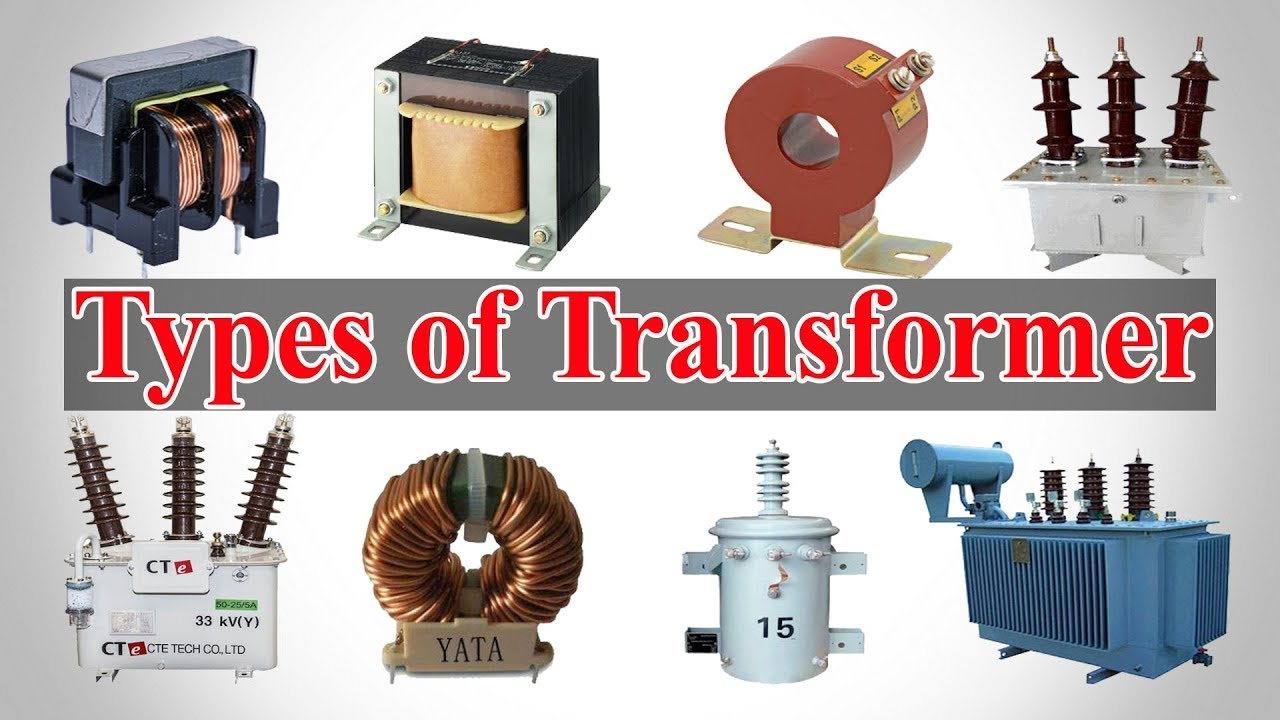
\includegraphics[width=\linewidth]{trafo.jpg}
            \caption[trafo]{Transformator}
        \end{figure}

    \end{columns}
\end{frame}

\begin{frame}{Pokok Bahasan}
    Pokok bahasan yang akan dijelaskan pada bab ini adalah 
    \begin{itemize}
        \item Induktansi bersama atau \emph{Mutual Inductance},
        \item Pemberian \emph{dot} pada suatu gambar rangkaian untuk menentukan polaritas tegangan dari komponen kopel,
        \item Linier transformator,
        \item Ideal tranformator,
        \item Ideal autotransformator, dan
        \item Transformator 3 fasa.
    \end{itemize}
\end{frame}

\section{Mutual Inductance}

\begin{frame}{Mutual Inductance}
    
    Ketika dua induktor atau koil cukup dekat, fluks magnetik yang disebabkan oleh arus pada koil satu terhadap koil lainnya, menyebabkan terjadinya induksi tegangan. \\~\\
    Fenomena ini disebut dengan \emph{Mutual Inductance} atau induktansi bersama
\end{frame}


\begin{frame}[standout]
    Ada Pertanyaan?
\end{frame}
  
\appendix
  
\end{document}